% \subsection{Anonymous Atomic Locks for coin mixing and cross-chain payments}
\subsection{Cryptocurrency Mixers}\label{sec:mixers}

\textit{(Parts of this section are taken/adapted from \cite{CCS:GMMMTT22}.)}

% \noemi{How to position this? Our focus will be on \emph{off-chain} mixers, whose focus is on enabling \emph{scalability} and \emph{interoperability} rather than privacy...}
% \todo{Talk about how these also solve scalability and interoperability?}

Cryptocurrency mixers~\cite{ESORICS:RufMorKat14,EPRINT:SNBB19,ACSAC:TLKBS18,FC:BNMCKF14,coinjoin,CCS:GreMie17} add a measure of $k$-anonymity to cryptocurrency tokens by employing a central party, or \emph{mixer}, to shuffle the tokens among users of the service. Users deposit their coins into the service, and later retrieve them again (using a different address, otherwise anonymity is trivially broken).
Any particular token (retrieved from the mixer) cannot be tied to a particular source (user who deposited money into the mixer): each of the $k$ users is equally likely to be the source of a given token. For security, a mixer must offer \emph{atomicity}, i.e., a user pays $c+\epsilon$ coins if and only if the ``recipient'' (normally the same user, but under a new address) is paid $c$ coins ($\epsilon$ is a parameter which represents the mixer and transaction fees).

When the underlying blockchain offers scripting functionality, a simple mixer can be set up as an account into which users deposit coins and later retrieve them (or allow another party to retrieve them) by redeeming a token, where atomicty is enforced via an on-chain script. When the goal is scalability and/or interoperability between different blockchains, more complicated protocols are needed to enforce the atomicity requirement without relying on the on-chain scripting functionality. 

\begin{figure}[htb]
    \centering
    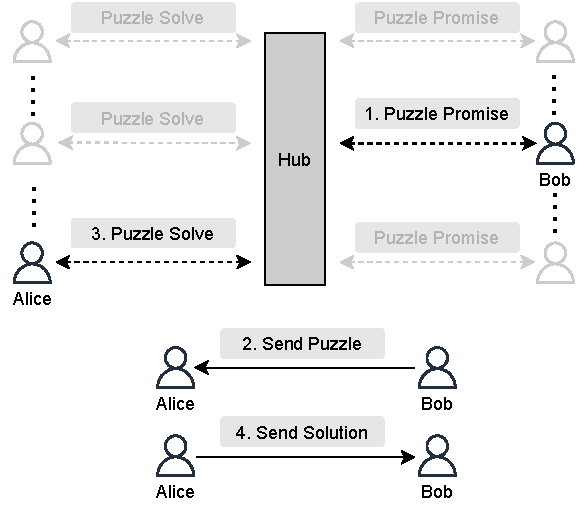
\includegraphics[width=0.7\linewidth]{syncpuzzle.pdf}
    \caption{Protocol flow of a synchronization puzzle, the un-
    derlying cryptographic mechanism of Tumblebit and \AAL, which we formalize as Blind Conditional Signatures.
    Dotted double-edged arrows indicate 2-party protocols. Solid arrows indicate secure point-to-point communication.}
    \label{fig:syncpuzzle_overview}
  \end{figure}

One line of work, initiated by TumbleBit~\cite{NDSS:HABSG17}, uses a protocol paradigm which we refer to as a \emph{synchronization puzzle}. A synchronization puzzle is a three-party protocol between a sender Alice, a mixer Hub, and a recipient Bob (\Cref{fig:syncpuzzle_overview}). Synchronization puzzle protocols consist of four steps: (1) Hub and Bob execute the \emph{puzzle promise} phase with respect to some message $m_{HB}$, which outputs a puzzle $\tau$ containing a hidden signature $\sigma_{HB}$ on $m_{HB}$. (2) Bob sends $\tau$ to Alice via a private channel, who (3) uses it to execute the \emph{puzzle solver} phase with Hub with respect to another message $m_{AH}$. At the end of this phase, Alice obtains the signature $\sigma_{HB}$ on $m_{HB}$ and Hub learns $\sigma_{AH}$ on $m_{AH}$. To conclude, (4) Alice sends $\sigma_{HB}$ to Bob. A synchronization puzzle protocol should satisfy the following properties:
\begin{itemize}
    \item \textbf{Blindness}: In the puzzle solver phase, Hub \emph{blindly} helps solve $\tau$, i.e., the phase should not reveal anything about $\tau$ to Hub. (This keeps Alice and Bob unlinkable from the point of view of Hub.)
    \item \textbf{Unlockability}: If the puzzle solver phase completes successfully, $s$ must be a valid secret for $\tau$. (This ensures that the Hub cannot learn $\sigma_{AH}$ without revealing $\sigma_{HB}$.)
    \item \textbf{Unforgeability}: Bob cannot output a valid signature $\sigma_{HB}$ on $m_{HB}$ before the puzzle solver phase completes. (This ensures Bob cannot learn $\sigma_{HB}$ without Hub learning $\sigma_{AH}$.)
\end{itemize}
To use a synchronization puzzle to realize an atomic payment, the parties set $m_{AH} : (A \xrightarrow{c+\epsilon} H)$ and $m_{HB} : (H \xrightarrow{c} B)$, where $(U_i \xrightarrow{c} U_j)$ denotes a payment of $c$ coins from user $U_i$ to $U_j$. Then $\sigma_{AH}$ and $\sigma_{HB}$ are set to the signatures authorizing $m_{AH}$ and $m_{HB}$, respectively. Thus, at the completion of the protocol Alice will have sent $c$ coins to Bob (and paid a fee of $\epsilon$ to Hub).

% Tumblebit realizes a synchronization puzzle via RSA encryption~\cite{RSA78} and hashed timelock contract (HTLCs), the latter of which is only present in certain ``scripting'' cryptocurrencies (e.g., Bitcoin and Ethereum).
% \noemi{RSA is used to encrypt the puzzle solution, and the ciphertext is rerandomized by Alice as in A2L. The HTLCs are used to extract the secret once the signature posted; A2L substitutes this with adaptor signatures.}

\subsubsection{Anonymous Atomic Locks (\texorpdfstring{\AAL}{A2L})}

A follow-up work~\cite{SP:TaiMorMaf21} introduces Anonymous Atomic Locks (\AAL), a protocol for off-chain coin mixing which requires only limited capabilities of the underlying blockchain, i.e., no scripting functionality.
Before we describe its approach to instantiating synchronization puzzles, we introduce the notion of \emph{adaptor signatures}, which will be used as a building block:

\begin{definition}[adaptor signature~\cite{AC:AEEFHM21}]
    An adaptor signature scheme $\Pi_\ADP := (\kgen, \presign, \prevrfy, \adapt, \vrfy, \ext)$ is defined with respect to a digital signature scheme $\Pi_\DS$ and an NP relation $\Rel$:
    \begin{description}
        \item[$\kgen(\secparam) \to (\vk, \sk)$:] The key generation algorithm is the same as in the underlying digital signature scheme, i.e., $\Pi_\DS.\kgen$.
        \item[$\presign(\sk, m, Y) \to \presig$:] The pre-signing algorithm takes as input a signing key $\sk$, message $m$, and instance $Y$ of the relation $\Rel$ and returns a pre-signature $\presig$.
        \item[$\prevrfy(\vk, m, Y, \presig) \to \{0, 1\}$:] The pre-verification algorithm checks that a pre-signature is well-formed.
        \item[$\adapt(\presig, y) \to \sigma$:] Given a witness $y$ for the instance $Y$, this algorithm adapts the pre-signature $\presig$ into a valid signature $\sigma$.
        \item[$\vrfy(\vk, m, \sigma) \to \{0, 1\}$:] The verification algorithm is the same as in the underlying digital signature scheme, i.e., $\Pi_\DS.\vrfy$.
        \item[$\ext(\presig, \sigma, Y) \to y$:] Given a pre-signature $\tilde{sigma}$ and a signature $\sigma$ generated with respect to some instance $Y$, the extract algorithm outputs the corresponding witness $y$ such that $(Y, y) \in \Rel$.
    \end{description}
\end{definition}

An adaptor signature scheme should satisfy the following properties: \emph{pre-signature correctness}, which guarantees that for all instances $Y \in \Lang_\Rel$ and honestly generated $\presig, \sigma$, the pre-signature and signature pass (pre-)verification and the extracted witness $y' \gets \ext(\presig, \sigma, Y)$ should satisfy $(Y, y') \in \Rel$; \emph{unforgeability}, which is a straightforward extension of the standard existential unforgeability notion (EUF-CMA) for digital signatures; \emph{pre-signature adaptability}, which states that for any $Y \in \Lang_\Rel$ and corresponding pre-signature $\presig$, pre-verification implies that $\presig$ can be adapted to a verifying signature $\sigma$; and \emph{witness extractability}, which says that it is difficult for an adversary to adapt an honestly-generated pre-signature $\presig$ into a signature $\sigma$ which verifies but where $y' \gets \ext(\presig, \sigma, Y)$ such that $(Y, y') \notin \Lang_\Rel$. We refer the reader to \cite{CCS:GMMMTT22} for formal definitions.

Anonymous Atomic Locks (\AAL)~\cite{SP:TaiMorMaf21} uses a rerandomizable CPA-secure encryption scheme $\Pi_\ENC$ and an adaptor signature scheme $\Pi_\ADP$ to realize a synchronization puzzle which is compatible with a wider range of cryptocurrencies. Specifically, the puzzle promise phase outputs to Bob a ciphertext $c \gets \Pi_\ENC.\enc(\ek_H, y)$ and a pre-signature $\presig_{HB}$ on $m_{HB}$ with respect to a discrete-log instance $Y := g^y$. Bob sends $(c, Y)$ to Alice, who rerandomizes them using fresh randomness $r$ to $(c', Y') := (\Pi_\ENC.\enc(\ek_H, y+r), g^y g^r)$. She can now use $Y'$ to produce a pre-signature $\presig_{AH}$ on $m_{AH}$ and executes the puzzle solver phase with Hub using $c', \presig_{AH}$. Hub can use $\sk_H$ to decrypt $c'$ and obtain $y' := y+r$, which it uses to complete the presignature into a full signature $\sigma_{AH}$ on $m_{AH}$ (thus completing the left side of the payment). This allows Alice to extract $y'$ via $\Pi_\ADP.\ext(\presig_{AH}, \sigma_{AH}, Y')$ and use her knowledge of $r$ to recover $y$, which she sends to Bob. Now Bob uses $y$ to adapt $\presig_{HB}$ to a full signature $\sigma_{HB}$ on $m_{HB}$, thereby completing the right side of the payment.

\cite{SP:TaiMorMaf21} defines an ideal functionality, which is reproduced as $\F_\BCS$ in \cite{CCS:GMMMTT22}, and gives a UC proof of security for \AAL:

\begin{theorem}[Main theorem~\cite{SP:TaiMorMaf21} (paraphrased)\footnote{As we will show, this theorem is incorrect.}]\label{thm:a2l}
    Let $\sf COM$ be a secure commitment scheme, $\NIZK$ be a non-interactive zero-knowledge proof, $\Pi_\DS$ be EUF-CMA-secure signature schemes, $\Rel$ be an NP-relation, $\Pi_\ADP$ be a secure adaptor signature scheme with respect to $\Pi_\DS$ and $\Rel$, and $\Pi_\ENC$ be a rerandomizable CPA-secure encryption scheme. Then \AAL UC-realizes the ideal functionality $\F_\BCS$ assuming anonymous guaranteed delivery channels and a synchronous network.
\end{theorem}

\subsubsection{Insecurity of \texorpdfstring{\AAL}{A2L}}\label{sec:a2l-attacks}

In \cite{CCS:GMMMTT22}, we analyzed the \AAL protocol~\cite{SP:TaiMorMaf21} and found that, in contrast to its claims, it is not secure. Although \AAL was proven secure in the universal composability (UC)~\cite{FOCS:Canetti01} framework, we show that a gap in their formal model allows two constructions which are completely insecure despite meeting their definitions: one admits a key recovery attack and the other allows a colluding sender and recipient to steal coins from the mixer. We will show how to close this gap in \cref{sec:bcs}.

In more detail, we show that there exist cryptographic primitives which satisfy the prerequisites of \AAL's main theorem, but allow \textit{(a)} a \emph{key recovery attack}, in which a malicious user is able to learn the long-term secret of the hub or \textit{(b)} a \emph{one-more signature attack}, in which a sender and recipient can collude to obtain $\secpar+1$ tokens from the hub while only sending $\secpar$ tokens. Both attacks run in polynomial time and succeed with overwhelming probability. These instantiations of \AAL are specifically crafted allow an attack and do not imply that all instantiations of \AAL are broken; however, we cannot prove the security of \AAL either. This tension is discussed further in \cref{sec:bcs}.

Below we give informal descriptions of both attacks. We refer the reader to \cite{CCS:GMMMTT22} for detailed descriptions and analysis. Both attacks rely on the fact that in the \AAL protocol, Hub offers a malicious Alice something very close to a decryption oracle. This oracle, which we refer to as $\oaal$, is programmed with a decryption key $\dk$ and takes as input a verification key $\vk$, message $m$, group element $h$, ciphertext $c$, and pre-signature $\presig$. It computes the plaintext $\tilde{x} \gets \Pi_\ENC.\dec(\dk, c)$ and attempts to use it to adapt $\presig$, i.e., computes $\sigma' \gets \Pi_\ADP.\adapt(\presig, \tilde{x})$. If it is successful, i.e., $\Pi_\ADP.\vrfy(\vk, m, \sigma') = 1$ or equivalently $\tilde{x} = x$, it returns $\sigma'$; otherwise it returns $\perp$. Note that the sender (Alice) can easily generate inputs to query the oracle: $\vk$ is the querier's own verification key, $m$ can be any arbitrary message in the message space, and generating $\presig$ that is valid when adapted with the (unknown) value $x$ requires only knowledge of the party's own signing key and a value $h = g^x$. The counterexamples below make use of the fact that $\sigma'$ implicitly reveals $\tilde{x} = \Pi_\ADP.\ext(\presig, \sigma, h)$. This leakage is not addressed in \AAL's proof of security.

\paragraph{Key recovery attack.} We show how to recover Hub's decryption key $\dk$ with $\secpar$ queries to $\oaal$ when \AAL is instantiated with an encryption scheme $\Pi_\ENC$ which, in addition to being re-randomizable and CPA-secure (as required by \Cref{thm:a2l}) has the following properties:
\begin{itemize}
    \item linearly homomorphic over $\ZZ_p$
    \item circular secure for bit encryption, i.e., CPA-secure even given the bitwise encryption of the decryption key
    \item the aforementioned ciphertexts $(c_1, \dots, c_\secpar) := (\enc(\ek, \dk_1), \dots, \enc(\ek,\allowbreak \dk_\secpar))$ are included in the encryption key $\ek$
\end{itemize}

Note that even with these additional assumptions, $\Pi_\ENC$ still satisfies the conditions of \Cref{thm:a2l}, and yet \AAL instantiated with such a scheme is insecure. In particular, a malicious Alice can use $\secpar$ queries to recover Hub's long-term decryption key $\dk$. The intuition of the attack is as follows: Alice samples a witness $x \sample \ZZ_p$ and computes the ciphertext $c \gets \Pi_\ENC.\enc(\ek, x)$. Now she can use the provided bitwise encryption of $\dk$ to homomorphically compute $c_i' := \Pi_\ENC.\enc(\ek, x + \dk_i)$ for each bit of the key. Getting the remaining inputs to the oracle is easy, since she can use her signing key to compute $h := g^x$ and $\presig \gets \Pi_\ADP.\presign(\sk, m, h)$ for an arbitrary $m$. At this point, she can query $\oaal(\vk_A, m, h, c_i, \presig)$ for $i = 1, \dots, \secpar$. The oracle returns $\perp$ if and only if $\dk_i = 1$, since $g^{x+1} \neq h = g^x$; otherwise, the oracle outputs an adapted signature $\sigma'$, and Alice learns that $\dk_i = 0$. This attack succeeds with probability 1. Recall that obtaining a non-$\perp$ response from the oracle is equivalent to authorizing a payment of $c$ coins from Alice to Hub, so it costs $nc \leq n\secpar$ coins (where $n$ is the number of 0 bits in $\dk$).

\paragraph{One-more signature attack.} Next, we show how to steal 1 coin from the hub for every $q \in O(\secpar)$ successful payments, i.e., learn $q+1$ signature witnesses for every $q$ non-$\perp$ queries to $\oaal$. This attack works when \AAL is instantiated with an encryption scheme $\Pi_\ENC$ which, in addition to being re-randomizable and CPA-secure (as required by \Cref{thm:a2l}) has the following properties:
\begin{itemize}
    \item linearly homomorphic over $\ZZ_p$
    \item supports homomorphic evaluation of the \emph{conditional bit flip} ($\sf CFlip$) function, defined as $\Pi_\ENC.\mathsf{CFlip}(\ek, i, \Pi_\ENC.\enc(\ek, x)) := \Pi_\ENC.\enc(\ek, y)$ where
    \[
        y = \begin{cases} 
            x &\text{ if } x[i] = 0\\ 
            x \oplus e_i &\text{ if } x[i] = 1
        \end{cases}
    \]
    Here $e_i$ is the $i$-th unit vector and $x[i]$ is the $i$th bit of $x$.
\end{itemize}
Again, even with these additional assumptions, $\Pi_\ENC$ still satisfies the conditions of \Cref{thm:a2l}, and yet \AAL instantiated with such a scheme is insecure. The intuition of the attack is as follows: given $q+1$ puzzle promise instances $(c_j := \Pi_\ENC.\enc(\ek, x_j), h_j := g^{x_j})$ for $j = 1, \dots, q+1$, Alice will attempt to learn the bits of $x_1$ by conditionally flipping them one at a time. Each query $i$ consists of a ciphertext $c'$ containing a random linear combination of the $c_j$'s, where $c_1$'s $i$th bit is also conditionally flipped, and $h'$ which is the same random linear combination of $h_j$'s \emph{without} $x_1$'s $i$th bit being conditionally flipped. If the oracle response is $\perp$, $c'$ and $h'$ were inconsistent which means the $i$th bit of $x_1$ was a 1. Otherwise, if the oracle responds with a non-$\perp$ value $y_i$, the $i$th bit of $x_1$ was a 0 and Alice has additionally learned the value of one random linear combination of the $x_j$'s. By the time $q = \sizeof{x_1}$ non-$\perp$ queries have been made, Alice has learned all the bits of $x_1$ and also has $\secpar$ linear equations with $\secpar$ unknowns. Since the coefficients are uniformly chosen, the equations are, with all but negligible probability, linearly independent; and since $\ZZ_p$ is a field, the solution is uniquely determined and can be found efficiently via Gaussian elimination. Furthermore, the length of each $x_i$ is $\secpar$, so the attack is efficient.

\subsubsection{Formalizing Blind Conditional Signatures}\label{sec:bcs}

In light of our attacks, the natural question is whether we can establish formally rigorous security guarantees for an (appropriately patched) \AAL protocol. While it seems unlikely that \AAL can achieve UC-security (more discussion on this later), we investigate whether it satisfies some weaker, but still meaningful, notion of security. Our main observation here is that a weak notion of CCA-security for encryption schemes suffices to provide formal guarantees for \AAL. This notion, which we refer to as \emph{one-more CCA-security}, (roughly) states that it is hard to recover the plaintexts of $n$ ciphertexts while querying a decryption oracle at most $n-1$ times. Importantly, this notion is, in principle, not in conflict with the homomorphism/re-randomization requirements, contrary to standard CCA-security.

To place the synchronization puzzle on firmer foundations, in \cite{CCS:GMMMTT22} we introduce a new primitive called blind conditional signtaures (BCS)\footnote{not to be confused with conditional blind signatures~\cite{EPRINT:ZacGroPag17}.} which captures the core synchronization puzzle functionality. We give game-based security definitions for BCS and show how to modify \AAL to obtain a new protocol, \AALplus, which meets these definitions. We also give a UC-secure construction of BCS, dubbed \AALUC, which requires much more complex machinery. In this section, we summarize the remaining contributions and constructions of~\cite{CCS:GMMMTT22}. 

\paragraph{Game-based definitions.} Towards establishing a formal analysis of \AAL, we introduce the notion of blind conditional signatures (BCS) which captures the core synchronization puzzle functionality. We propose game-based definitions similar in spirit to the well-established security definitions of regular blind signatures~\cite{C:Chaum82,JC:SchUnr17}. 

\begin{definition}[Blind Conditional Signature]
    A blind conditional signature $\Pi_\mathsf{BCS}\allowbreak :=(\setup, \Promise, \Pay, \Open)$ is defined with respect to a signature scheme $\Pi_\DS := (\kgen,\sign,\vrfy)$ and consists of the following efficient algorithms.
    
    \begin{itemize}%[leftmargin=*]
    \item {$(\tilde{\ek}, \tilde{\dk})\gets \setup(\secparam)$}: The setup algorithm takes as input the security parameter $\secparam$ and outputs a key pair $(\tilde{\ek}, \tilde{\dk})$.
    \item {$(\bot, \{\tau, \bot\}) \gets \Promise \left\langle \begin{matrix} H \left(\tilde{\dk}, \sk^H, m_{HB} \right)\\ B \left(\tilde{\ek}, \vk^H, m_{HB} \right) \end{matrix} \right\rangle $}: The puzzle promise algorithm is an interactive protocol between two users $H$ (with inputs the decryption key $\tilde{\dk}$, the signing key $\sk^H$, and a message $m_{HB}$) and $B$ (with inputs the encryption key $\tilde{\ek}$, the verification key $\vk^H$, and a message $m_{HB}$)  and returns $\bot$ to $H$ and either a puzzle $\tau$ or $\bot$ to $B$.
    \item {$(\{(\sigma^*, s), \bot\}, \{\sigma^*, \bot\}) \gets \Pay \left\langle \begin{matrix} A \left(\sk^A, \tilde{\ek}, m_{AH}, \tau\right)\\ H \left(\tilde{\dk}, \vk^A, m_{AH} \right) \end{matrix} \right\rangle $}: The puzzle solving algorithm is an interactive protocol between two users $A$ (with inputs the signing key $\sk^A$, the encryption key $\tilde{\ek}$, a message $m_{AH}$, and a puzzle $\tau$) and $H$ (with inputs the decryption key $\tilde \dk$, the verification key $\vk^A$, and a message $m_{AH}$) and returns to both users either a signature $\sigma^*$ ($A$ additionally receives a secret $s$) or $\bot$.
    \item {$\{\sigma, \bot\}\gets \Open(\tau, s)$}: The open algorithm takes as input a puzzle $\tau$ and a secret $s$ and returns a signature $\sigma$ or $\bot$.
    \end{itemize}
\end{definition}

Informally, correctness holds if for all honest executions of the protocols, the resulting signatures $\sigma$ and $\sigma^*$ verify.

% Next, we define correctness.
% \begin{definition}[Correctness]
%     A blind conditional signature $\Pi_\mathsf{BCS}$ is correct if for all $\secpar\in \mathbb{N}$, all $(\tilde{\ek}, \tilde{\dk})$ in the support of $\setup(\secparam)$, all $(\vk^H, \sk^H)$ and $(\vk^A, \sk^A)$ in the support of $\Pi_\DS.\kgen(\secparam)$, and all pairs of messages $(m_{HB}, m_{AH})$, it holds that
%     $$
%     \Pr\left[\vrfy(\vk^H,m_{HB}, \Open(\tau, s)) = 1\right] = 1
%     $$
%     and
%     $$
%     \Pr\left[\vrfy(\vk^A,m_{AH}, \sigma^*) = 1\right] = 1
%     $$
%     where 
%     \begin{itemize}%[leftmargin=*]
%         \item $\tau \gets \Promise \left\langle \begin{matrix} H \left(\tilde{\dk}, \sk^H, m_{HB} \right)\\ B \left(\tilde{\ek}, \vk^H, m_{HB}\right) \end{matrix} \right\rangle$ and
%         \item $((\sigma^*, s), \sigma^*) \gets \Pay \left\langle \begin{matrix} A \left(\sk^A,  \tilde{\ek}, m_{AH}, \tau\right)\\ H \left(\tilde{\dk}, \vk^A, m_{AH}\right) \end{matrix} \right\rangle$.
%     \end{itemize}
% \end{definition}
%

The game-based security guarantees of BCS consist of three properties:
\begin{description}
    \item[Blindness.] Our definition of blindness is akin to the strong blindness notion of standard blind signatures~\cite{C:Chaum82}, in which the adversary picks the keys (as opposed to the weak version in which they are chosen by the experiment)\footnote{We opt for this stronger version since we want to provide anonymity even in the case of a fully malicious hub, which can pick its keys adversarially to try to link a sender/receiver pair.}. Roughly speaking, it says that two promise/solve sessions cannot be linked together by the hub.\footnote{We do not consider the case in which Hub colludes with either Alice or Bob, since deanonymization is trivial (Alice (resp. Bob) simply reveals the identity of Bob (resp. Alice) to Hub); this is in line with \cite{SP:TaiMorMaf21}.}\footnote{In previous works, descriptions of unlinkability assume an explicit step for blinding the puzzle $\tau$ between $\Promise$ and $\Pay$. Here, we assume that $\Pay$ performs this blinding functionality.}
    % \begin{definition}[Blindness]
    %     A blind conditional signature $\Pi_\BCS$ is blind if there exists a negligible function $\negl$ such that for all $\secpar \in \NN$ and all PPT adversaries $\adv$, the following holds:
    %     \[ \prob{\expUnlink^{\adv}_{\Pi_{\mathsf{puzzle}}}(\secpar) = 1} \le \frac{1}{2} + \negl\]
    %     where $\expUnlink$ is defined in~\cref{fig:exp_unlinkability}.\footnote{In previous works, descriptions of unlinkability assume an explicit step for blinding the puzzle $\tau$ between $\Promise$ and $\Pay$. Here, we assume that $\Pay$ performs this blinding functionality.}
    % \end{definition}
    \item[Unlockability.] This property says that it should be hard for Hub to create a valid signature on Alice's message that does not allow Bob to unlock the full signature in the corresponding promise session.
    % \begin{definition}[Unlockability]
    %     A blind conditional signature $\Pi_\mathsf{BCS}$ is unlockable if there exists a negligible function $\negl$ such that for all $\secpar \in \NN$ and all PPT adversaries $\adv$, the following holds:
    %     \[ \prob{\expUnlock^{\adv}_{\Pi_{\mathsf{BCS}}}(\secpar) = 1} \le \negl\]
    %     where $\expUnlock$ is defined in~\cref{fig:exp_unlockability}.
    % \end{definition}
    \item[Unforgeability.] Our definition of unforgeability is inspired by the unforgeability of blind signatures~\cite{C:Chaum82}. We require that Alice and Bob cannot recover $q$ signatures from Hub while successfully querying the solving oracle at most $q-1$ times. Since each successful query reveals a signature from Alice's key (which in turn corresponds to a transaction from Alice to Hub), this requirement implicitly captures the fact that Alice and Bob cannot steal coins from Hub. The winning condition $b_0$ captures the scenario where the adversary forges a signature of the hub on a message previously not used in any promise oracle query.
    The remaining conditions $b_1, b_2$ and $b_3$ together capture the scenario in which the adversary outputs $q$ valid distinct key-message-signature tuples while having queried for solve only $q-1$ times. Hence, in the second condition, the attacker manages to \emph{complete} $q$ promise interactions with only $q-1$ solve interactions, whereas in the first winning condition, the adversary computes a \emph{fresh} signature that is not the completion of any promise interaction. These conditions are technically incomparable: an attacker that succeeds under one condition does not imply an attacker succeeding on the other.
    It is important to note that this is different from the unforgeability notion of blind signatures (where the attacker only has access to a single signing oracle), since in our case the hub is offering the attacker two oracles: promise and solve.
    % \begin{definition}[Unforgeability]
    % A blind conditional signature $\Pi_\mathsf{BCS}$ is \emph{unforgeable} if there exists a negligible function $\negl$ such that for all $\secpar \in \NN$ and all PPT adversaries $\adv$, the following holds:
    % \begin{equation*}
    %      \prob{\expSec^{\adv}_{\Pi_{\mathsf{BCS}}}(\secpar) = 1} \le \negl
    % \end{equation*}
    % where $\expSec$ is defined in~\cref{fig:exp_security_ab}.
    % \end{definition}
\end{description}

%     \begin{figure}
        \centering
        \makebox[0pt]{\begin{minipage}{1.35\textwidth}
        \begin{pchstack}[boxed]
        \begin{pcvstack}
        %%%%%%%%%%%%%%%%%%%%%%%%%%%%%%%%%%%%%
        %%%%% Blindness (unlinkability) %%%%%
        %%%%%%%%%%%%%%%%%%%%%%%%%%%%%%%%%%%%%
        \begin{pchstack}%[boxed]
        \procedure[space=auto,codesize=\small]{Blindness experiment $\expUnlink^{\adv}_{\Pi_{\mathsf{BCS}}}(\secpar)$}{
        \hfill\\[-0.5\baselineskip]
       (\tilde{\ek}, \vk^H_0, \vk^H_1, (m_{HB,0}, m_{AH,0}), (m_{HB,1}, m_{AH,1})) \gets \adv(\secparam)\\
        (\vk_0^A, \sk_0^A) \gets \kgen(\secparam)\\
        (\vk_1^A, \sk_1^A) \gets \kgen(\secparam)\\
        \tau_0 \gets \Promise \left\langle  \adv(\vk_0^A, \vk_1^A), \bob(\tilde{\ek}, \vk^H_0, m_{HB,0}) \right\rangle\\
        \tau_1 \gets \Promise \left\langle  \adv(\vk_0^A, \vk_1^A), \bob(\tilde{\ek}, \vk^H_1, m_{HB,1}) \right\rangle\\
        b \gets \{0,1\}\\
        (\sigma^*_0, s_0) \gets \Pay \left\langle  \alice \left(\sk_0^A, \tilde{\ek}, m_{AH,0}, \tau_{0 \oplus b}\right), \adv \right\rangle \\
        (\sigma^*_1, s_1) \gets \Pay \left\langle  \alice \left(\sk_1^A, \tilde{\ek}, m_{AH,1}, \tau_{1 \oplus b}\right), \adv \right\rangle \\
        \mathbf{if~}(\sigma^*_0 = \bot) \lor (\sigma^*_1 = \bot) \lor (\tau_0 = \bot) \lor (\tau_1 = \bot)\\
        \quad \sigma_0 := \sigma_1 := \bot\\
        \mathbf{else}\\
        \quad \sigma_{0 \oplus b} \gets \Open(\tau_{0 \oplus b}, s_0)\\
        \quad \sigma_{1 \oplus b} \gets \Open(\tau_{1 \oplus b}, s_1)\\
        b' \gets \adv(\sigma_0, \sigma_1)\\
        \mathbf{return}\ (b = b')
        }
        \end{pchstack}
        \pcvspace
        %%%%%%%%%%%%%%%%%%%%%%%%%%%%%%%%%%%%%
        %%%%%      Unlockability        %%%%%
        %%%%%%%%%%%%%%%%%%%%%%%%%%%%%%%%%%%%%
        \begin{pchstack}%[boxed]
        \procedure[space=auto,codesize=\small]{Unlockability experiment $\expUnlock^{\adv}_{\Pi_{\mathsf{BCS}}}(\secpar)$}{
        \hfill\\[-0.5\baselineskip]
        (\tilde{\ek}, \vk^H, m_{HB}, m_{AH}) \gets \adv(\secparam)\\
        (\vk^A, \sk^A) \gets \kgen(\secparam)\\
        \tau \gets \Promise \left\langle  \adv(\vk^A), \bob(\tilde{\ek}, \vk^H, m_{HB}) \right\rangle\\
        \textbf{if } \tau = \bot\\
        \quad (\hat{\sigma}, \hat{m}) \gets \adv\\ 
        \quad b_0 := (\vrfy(\vk^A,\hat{\sigma}, \hat{m}) =1)\\
        \textbf{if } \tau \neq \bot\\
            \quad (\sigma^*,s) \gets \Pay \left\langle  \alice \left(\sk^A, \tilde{\ek}, m_{AH},\tau\right), \adv \right\rangle\\
        \quad (\hat{\sigma}, \hat{m}) \gets \adv\\ 
        \quad b_1 := (\vrfy(\vk^A,\hat{\sigma}, \hat{m}) =1) \land (\hat{m} \neq m_{AH})\\
         \quad b_2 := (\vrfy(\vk^A,\sigma^*, m_{AH}) =1)\\
        \quad b_3 := (\vrfy(\vk^H, m_{HB}, \Open(\tau,s)) \neq1) \\
         \mathbf{return}\ b_0 \lor b_1 \lor (b_2 \land b_3)
        }
        \end{pchstack}
        \end{pcvstack}
        \pchspace
        %%%%%%%%%%%%%%%%%%%%%%%%%%%%%%%%%%%%%
        %%%%%      Unforgeability       %%%%%
        %%%%%%%%%%%%%%%%%%%%%%%%%%%%%%%%%%%%%
        \begin{pchstack}%[boxed]
        \begin{pcvstack}
        \procedure[space=auto,codesize=\small]{Unforgeability experiment $\expSec^{\adv}_{\Pi_{\mathsf{BCS}}}(\secpar)$}{
        \hfill\\[-0.5\baselineskip]
    \mathcal{L} := \emptyset, Q := 0 \\
    (\tilde{\ek}, \tilde{\dk}) \gets \setup(\secparam)\\
    (\vk_1^H, m_1, \sigma_1), \ldots, (\vk_q^H, m_q, \sigma_q)  \gets \adv^{\oracle\mathsf{PP}(\cdot), \oracle\mathsf{PS}(\cdot)}(\tilde{\ek})\\
    b_0 := \exists i \in [q] \suchthat (\vk_i^H,\cdot) \in \mathcal{L} \land (\vk_i^H,m_i) \notin \mathcal{L} \\
    \qquad \qquad  \land \vrfy(\vk_i^H,m_i,\sigma_i) = 1\\
    b_1 := \forall i \in [q], (\vk_i^H,m_i) \in \mathcal{L} \land \vrfy(\vk_i^H, m_i, \sigma_i) = 1\\
    b_2 := \bigwedge_{i,j \in [q], i \ne j}  (\vk_i^H, m_i, \sigma_i) \ne (\vk_j^H, m_j, \sigma_j) \\
    b_3 := (Q \le q-1) \\
    \mathbf{return}\ b_0 \lor (b_1 \land b_2 \land b_3)
    }
    \pcvspace
    
    \procedure[space=auto,codesize=\small]{$\oracle\mathsf{PP}(m)$}{
    \hfill\\[-0.5\baselineskip]
    (\vk^H, \sk^H) \gets \Pi_\ADP.\kgen(\secparam)\\
    \mathcal{L} := \mathcal{L} \cup \{ (\vk^H,m) \}\\
    \bot \gets \Promise\langle H(\tilde{\dk}, \sk^H, m), \adv(\vk^H) \rangle \\
    }
    
    
    \procedure[space=auto,codesize=\small]{$\oracle\mathsf{PS}(\vk^A, m')$}{
    \hfill\\[-0.5\baselineskip]
    \sigma^* \gets \Pay\langle \adv, H(\tilde{\dk}, \vk^A, m') \rangle \\
    \mathbf{if}\ \sigma^* \ne \bot\ \mathbf{then}~ Q:= Q+ 1
    }
        \end{pcvstack}
    \end{pchstack}
    \end{pchstack}
    \end{minipage}}
    \caption{BCS security games \label{fig:bcs_games}}
    \end{figure}
%
    % \begin{figure}
    %     \centering
    %     \begin{pchstack}[boxed]
    %     \procedure[space=auto,codesize=\small]{$\expUnlock^{\adv}_{\Pi_{\mathsf{BCS}}}(\secpar)$}{
    %     \hfill\\[-0.5\baselineskip]
    %     (\tilde{\ek}, \vk^H, m_{HB}, m_{AH}) \gets \adv(\secparam)\\
    %     (\vk^A, \sk^A) \gets \kgen(\secparam)\\
    %     \tau \gets \Promise \left\langle  \adv(\vk^A), \bob(\tilde{\ek}, \vk^H, m_{HB}) \right\rangle\\
    %     \textbf{if } \tau = \bot\\
    %     \quad (\hat{\sigma}, \hat{m}) \gets \adv\\ 
    %     \quad b_0 := (\vrfy(\vk^A,\hat{\sigma}, \hat{m}) =1)\\
    %     \textbf{if } \tau \neq \bot\\
    %         \quad (\sigma^*,s) \gets \Pay \left\langle  \alice \left(\sk^A, \tilde{\ek}, m_{AH},\tau\right), \adv \right\rangle\\
    %     \quad (\hat{\sigma}, \hat{m}) \gets \adv\\ 
    %     \quad b_1 := (\vrfy(\vk^A,\hat{\sigma}, \hat{m}) =1) \land (\hat{m} \neq m_{AH})\\
    %      \quad b_2 := (\vrfy(\vk^A,\sigma^*, m_{AH}) =1)\\
    %     \quad b_3 := (\vrfy(\vk^H, m_{HB}, \Open(\tau,s)) \neq1) \\
    %      \mathbf{return}\ b_0 \lor b_1 \lor (b_2 \land b_3)
    %     }
    % \end{pchstack}
    %     \caption{Unlockability experiment} 
    %     \label{fig:exp_unlockability}
    % \end{figure}
    % %
    % \begin{figure}
    %     \centering
    %     \begin{pchstack}[boxed]
    %     \begin{pcvstack}
    %     \procedure[space=auto,codesize=\small]{$\expSec^{\adv}_{\Pi_{\mathsf{BCS}}}(\secpar)$}{
    %     \hfill\\[-0.5\baselineskip]
    % \mathcal{L} := \emptyset, Q := 0 \\
    % (\tilde{\ek}, \tilde{\dk}) \gets \setup(\secparam)\\
    % (\vk_1^H, m_1, \sigma_1), \ldots, (\vk_q^H, m_q, \sigma_q)  \gets \adv^{\oracle\mathsf{PP}(\cdot), \oracle\mathsf{PS}(\cdot)}(\tilde{\ek})\\
    % b_0 := \exists i \in [q] \suchthat (\vk_i^H,\cdot) \in \mathcal{L} \land (\vk_i^H,m_i) \notin \mathcal{L} \\
    % \qquad \qquad  \land \vrfy(\vk_i^H,m_i,\sigma_i) = 1\\
    % b_1 := \forall i \in [q], (\vk_i^H,m_i) \in \mathcal{L} \land \vrfy(\vk_i^H, m_i, \sigma_i) = 1\\
    % b_2 := \bigwedge_{i,j \in [q], i \ne j}  (\vk_i^H, m_i, \sigma_i) \ne (\vk_j^H, m_j, \sigma_j) \\
    % b_3 := (Q \le q-1) \\
    % \mathbf{return}\ b_0 \lor (b_1 \land b_2 \land b_3)
    % }
    % \pcvspace
    
    % \procedure[space=auto,codesize=\small]{$\oracle\mathsf{PP}(m)$}{
    % \hfill\\[-0.5\baselineskip]
    % (\vk^H, \sk^H) \gets \Pi_\ADP.\kgen(\secparam)\\
    % \mathcal{L} := \mathcal{L} \cup \{ (\vk^H,m) \}\\
    % \bot \gets \Promise\langle H(\tilde{\dk}, \sk^H, m), \adv(\vk^H) \rangle \\
    % }
    
    
    % \procedure[space=auto,codesize=\small]{$\oracle\mathsf{PS}(\vk^A, m')$}{
    % \hfill\\[-0.5\baselineskip]
    % \sigma^* \gets \Pay\langle \adv, H(\tilde{\dk}, \vk^A, m') \rangle \\
    % \mathbf{if}\ \sigma^* \ne \bot\ \mathbf{then}~ Q:= Q+ 1
    % }
    %     \end{pcvstack}
    % \end{pchstack}
    %     \caption{Unforgeability experiment}
    %     \label{fig:exp_security_ab}
    % \end{figure}
    

% The security games are given in \Cref{fig:bcs_games}. We define security as the collection of all three properties:
We refer the reader to \cite{CCS:GMMMTT22} for the security games. Security is defined as the collection of all three properties:

\begin{definition}[Security]
    A blind conditional signature $\Pi_\mathsf{BCS}$ is secure if it is blind, unlockable, and unforgeable. %, i.e., if there exist negligible functions $\negln{1}, \negln{2}, \negln{3}$ such that for all $\secpar \in \NN$ and all PPT adversaries $\adv$, all of the following hold:
    % \begin{align*}
    %     \prob{\expUnlink^{\adv}_{\Pi_{\mathsf{puzzle}}}(\secpar) = 1} &\le \frac{1}{2} + \neglnf{1}\\
    %     \prob{\expUnlock^{\adv}_{\Pi_{\mathsf{BCS}}}(\secpar) = 1} &\le \neglnf{2}\\
    %     \prob{\expSec^{\adv}_{\Pi_{\mathsf{BCS}}}(\secpar) = 1} &\le \neglnf{3}
    % \end{align*}
\end{definition}    

\paragraph{The \AALplus protocol: a secure version of \AAL.}
With the BCS formalism in place, we can prove that an appropriately modified version of \AAL, which we call \AALplus, satisfies the above definitions. Our analysis comes with an important caveat: we analyze the security of our scheme in the \emph{linear-only encryption model}. This is a model introduced by Groth~\cite{TCC:Groth04} that only models adversaries that are restricted to perform ``legal'' operations on ciphertexts, similarly to the generic/algebraic group model. While this is far from a complete analysis, it increases our confidence in the security of the system.\footnote{We resort to the LOE model because of the seemingly inherent conflict between linear homomorphism and CCA-like security, both of which are needed for our application (in our setting, the adversary has access to something akin to a decryption oracle). Indeed, even proving that ElGamal encryption is CCA1-secure in the standard model is a long-standing open problem, and we believe that the \AAL approach would inherently hit this barrier without some additional assumption.} We defer the details of the \AALplus protocol, its analysis, and a discussion of its overhead with respect to \AAL to \cite{CCS:GMMMTT22}.

% \newcommand{\blue}[1]{\textcolor{blue}{#1}}
\newcommand{\green}[1]{\textcolor{teal}{#1}}
\newcommand{\twoPC}{\ensuremath{\mathsf{2PC}}}

\begin{figure*}%[!t]
\centering
%\resizebox{\textwidth}{!}{
\makebox[0pt]{\begin{minipage}{1.4\textwidth}
%%%%%%%%%%%%%%%%%%%%%%%%%%%%%%%%%
%%%%%%    PUZZLE PROMISE    %%%%%
%%%%%%%%%%%%%%%%%%%%%%%%%%%%%%%%%
\begin{pchstack}[boxed]
    \procedure{Public parameters: group description $(\GG, g, q)$, message $m_{HB}$}{
 	\text{ $\Promise \langle H( \dk_H, \sk_{HB}^H), \cdot \rangle$} \< \< \text{$\Promise \langle \cdot, B(\ek_H, \vk_{HB}^H) \rangle$} \\[][\hline]
	\pcln s \sample \ZZ_p, Y := g^s \< \< \\ [-0.15\baselineskip][]
	\pcln c \gets \Pi_\ENC.\enc(\ek_H, s) \< \< \\ [-0.15\baselineskip][]
	\pcln \pi_s \gets \NIZK.\prove( (\ek_H, Y, c), s)  \< \< \\ [-0.15\baselineskip][]
	\pcln \tilde{\sigma}_{HB}^H \gets \Pi_\ADP.\presig( \sk_{HB}^H, m_{HB}, Y ) \< \< \\ [-0.85\baselineskip][]
	\pcln \< \sendmessageright*{Y, c, \pi_s, \tilde{\sigma}_{HB}^H}\< \\ [-0.55\baselineskip][]
	\pcln \< \< {\mathbf{If}\ \NIZK.\vrfy((\ek_H,Y,c), \pi_s) \neq 1\ \mathbf{ then}\ \pcreturn \bot} \\ [-0.15\baselineskip][]
	\pcln \< \< \mathbf{If}\ \Pi_\ADP.\prevrfy(\vk_{HB}^H, m_{HB}, Y, \tilde{\sigma}_{HB}^H) \neq 1\ \mathbf{then} \\ [-0.15\baselineskip][]
	\pcln \< \< \quad \pcreturn \bot \\ [-0.15\baselineskip][]
	\pcln \< \< \mathbf{set}\ \tau := (m_{HB}, \tilde{\sigma}_{HB}^H, (Y, c)) \\ [-0.15\baselineskip][]
	\pcln \pcreturn \bot \< \< \pcreturn \tau
}
\end{pchstack}
%%%%%%%%%%%%%%%%%%%%%%%%%%%%%%%%%
%%%%%%     PUZZLE SOLVER    %%%%%
%%%%%%%%%%%%%%%%%%%%%%%%%%%%%%%%%
\begin{pchstack}[boxed]
    \procedure{Public parameters: group description $(\GG, g, q)$, message $m_{AH}$}{ 
 	\text{$\Pay \langle A(\sk_{AH}^A, \ek_H, \tau), \cdot\rangle$} \< \< \text{$\Pay \langle \cdot, H(\dk_H, \vk_{AH}^A) \rangle$} \\[][\hline]
 	\pcln \pcparse \tau := ( \cdot, \cdot, (Y, c)) \< \< \\ [-0.15\baselineskip][]
 	\pcln r \sample \ZZ_p, Y' := Y \cdot g^r \< \< \\ [-0.15\baselineskip][]
 	\pcln \tilde{\sigma}_{AH}^A \gets \Pi_\ADP.\presig( \sk_{AH}^A, m_{AH}, Y') \< \< \\ [-0.85\baselineskip][] 
 	\pcln \< \sendmessageright*{Y', \tilde{\sigma}_{AH}^A} \< \\ [-0.55\baselineskip][]
 	\pcln \< \< \mathbf{If}\ \Pi_\ADP.\prevrfy(\vk_{AH}^A, m_{AH}, Y', \tilde{\sigma}_{AH}^A) \neq 1\ \mathbf{then} \\ [-0.15\baselineskip][]
 	\< \< \quad \pcreturn \bot\\ [-0.15\baselineskip][]
 	\pcln \< \begin{subprocedure}
 	\dbox{\procedure[linenumbering]{$\twoPC((r,c), (\dk_H))$}{
 	\pcif \ek_H \neq \Pi_\ENC.\mathsf{Gen}(\dk_H)\\
 	\pcthen \text{abort}\\
 	s^* \gets \Pi_\ENC.\dec(\dk_H, c)\\
 	z := s^* + r\\
 	\pcreturn ((\bot), (z))
 	}}
 	\end{subprocedure}
 	\< \\ [-0.15\baselineskip][]
 	\pcln \< \< \mathbf{If}\ Y' \neq g^z\ \mathbf{then}\ \pcreturn \bot\\ [-0.15\baselineskip][]
 	\pcln \< \< \sigma_{AH}^A \gets \Pi_\ADP.\adapt(\tilde{\sigma}_{AH}^A, z)\\ [-0.85\baselineskip][]
 	%\pcln \< \< \sigma_{AH}^H \gets \Pi_\sign(\sk_{AH}^H, m)\\ [-0.85\baselineskip][]
 	\pcln \< \sendmessageleft*{{\sigma}_{AH}^A} \< \\ [-0.55\baselineskip][]
 	\pcln \mathbf{If}\ \Pi_\ADP.\vrfy(\vk_{AH}^A, m_{AH}, \sigma_{AH}^A) \neq 1\ \mathbf{then} \< \< \\ [-0.15\baselineskip][]
 	\pcln \quad \pcreturn \bot \< \< \\ [-0.15\baselineskip][]
 	\pcln z' \gets \Pi_\ADP.\ext(\tilde{\sigma}_{AH}^A, \sigma_{AH}^A, Y')\< \< \\ [-0.15\baselineskip][]
 	\pcln s := z'-r \< \< \\ [-0.15\baselineskip][]
 	\pcln \pcreturn (\sigma_{AH}^A, s) \< \< \pcreturn \sigma_{AH}^A
}
\end{pchstack}
%%%%%%%%%%%%%%%%%%%%%%%%%%%%%%%%%
%%%%%%     SETUP & OPEN     %%%%%
%%%%%%%%%%%%%%%%%%%%%%%%%%%%%%%%%
\begin{center}
    \begin{pchstack}[boxed]
        \procedure[space=auto,codesize=\small]{$\setup(\secparam)$}{
    (\ek_H, \dk_H) \gets \Pi_\ENC.\kgen(\secparam)\\
    \pcreturn (\ek_H, \dk_H)
    }
    
    \pchspace
    
    \procedure[space=auto,codesize=\small]{$\open(\tau, s)$}{
    \mathbf{parse}\ \tau := ( \cdot, \tilde{\sigma}, \cdot)\\
    \sigma \gets \Pi_\ADP.\adapt(\tilde \sigma, s)\\
    \pcreturn \sigma
    }
    \end{pchstack}
\end{center}
\end{minipage}}
%}
\caption{Puzzle promise, puzzle solver, and open protocols of \AALUC}
\label{fig:a2l_uc}
\end{figure*}

% \begin{figure}
%     \centering
%     \begin{pchstack}[boxed]
%         \procedure[space=auto,codesize=\small]{$\setup(\secparam)$}{
%     (\ek_H, \dk_H) \gets \Pi_\ENC.\kgen(\secparam)\\
%     \mathbf{set}\ \tilde \pk := \ek_H, \tilde \sk := \dk_H\\
%     \pcreturn (\tilde \pk, \tilde \sk)
%     }
    
%     \pchspace
    
%     \procedure[space=auto,codesize=\small]{$\open(\tau, s)$}{
%     \mathbf{parse}\ \tau := ( \cdot, \tilde{\sigma}, \cdot)\\
%     \sigma \gets \Pi_\ADP.\adapt(\tilde \sigma, s)\\
%     \pcreturn \sigma
%     }
%     \end{pchstack}
%     \caption{Setup and Open algorithms of our conditional puzzle construction}
%     \label{fig:our_protocol_algorithms}
% \end{figure}

% \begin{figure*}[h]
% \centering
% %\resizebox{\textwidth}{!}{
% \begin{pchstack}[boxed]
%     \procedure{Public parameters: group description $(\GG, g, q)$, message $m_{HB}$}{ 
%  	\text{ $\Promise \langle H( \dk_H, \sk_{HB}^H), \cdot \rangle$} \< \< \text{$\Promise \langle \cdot, B(\ek_H, \vk_{HB}^H) \rangle$} \\[][\hline]
% 	\pcln s \sample \ZZ_p, Y := g^s \< \< \\ [-0.15\baselineskip][]
% 	\pcln c \gets \Pi_\ENC.\enc(\ek_H, s) \< \< \\ [-0.15\baselineskip][]
% 	\pcln \pi_s \gets \NIZK.\prove( (\ek_H, Y, c), s)  \< \< \\ [-0.15\baselineskip][]
% 	\pcln \tilde{\sigma}_{HB}^H \gets \Pi_\ADP.\presig( \sk_{HB}^H, m_{HB}, Y ) \< \< \\ [-0.85\baselineskip][]
% 	\pcln \< \sendmessageright*{Y, c, \pi_s, \tilde{\sigma}_{HB}^H}\< \\ [-0.55\baselineskip][]
% 	\pcln \< \< {\mathbf{If}\ \NIZK.\vrfy((\ek_H,Y,c), \pi_s) \neq 1\ \mathbf{ then}\ \pcreturn \bot} \\ [-0.15\baselineskip][]
% 	\pcln \< \< \mathbf{If}\ \Pi_\ADP.\prevrfy(\vk_{HB}^H, m_{HB}, Y, \tilde{\sigma}_{HB}^H) \neq 1\ \mathbf{then} \\ [-0.15\baselineskip][]
% 	\pcln \< \< \quad \pcreturn \bot \\ [-0.15\baselineskip][]
% 	\pcln \< \< \mathbf{set}\ \tau := (m_{HB}, \tilde{\sigma}_{HB}^H, (Y, c)) \\ [-0.15\baselineskip][]
% 	\pcln \pcreturn \bot \< \< \pcreturn \tau
% % 	\pcln \< \< \text{If } \NIZK.\vrfy(\pi_s, (Y,c)) \neq 1 \text{ then abort} \\ [-0.15\baselineskip][]
% % 	\pcln \< \< \pcsend\ (Y, c)\ \pcto\ A \\ [-0.15\baselineskip][]
% % 	\pcln \< \< \pcreceive\ s^*\ \pcfrom\ A \\ [-0.15\baselineskip][]
% % 	\pcln \< \< \sigma_{HB}^H \gets \Pi_\ADP.\adapt(\tilde{\sigma}_{HB}^H, s^*) \\ [-0.15\baselineskip][]
% % 	\pcln \< \< \sigma_{HB}^B \gets \Pi_\DS.\sign(\sk_{HB}^B, m_{HB}) \\ [-0.15\baselineskip][]
% % 	\pcln \< \< \pcpost\ (m_{HB}, [\sigma_{HB}^H, \sigma_{HB}^B])\ \pcto\ \BB\\ [-0.15\baselineskip][]
% % 	\pcln \pcreturn \top \< \< \pcreturn \top 
% }
% \end{pchstack}
% %}
% \vspace{-0.2cm}
% \caption{Puzzle promise protocol of \sysnameuc}
% \label{fig:our_protocol_hub_bob}
% \vspace{-0.4cm}
% \end{figure*}

% \begin{figure*}
% \centering
% %\resizebox{\textwidth}{!}{
% \begin{pchstack}[boxed]
%     \procedure{Public parameters: group description $(\GG, g, q)$, message $m_{AH}$}{ 
%  	\text{$\Pay \langle A(\sk_{AH}^A, \ek_H, \tau), \cdot\rangle$} \< \< \text{$\Pay \langle \cdot, H(\dk_H, \vk_{AH}^A) \rangle$} \\[][\hline]
%  	\pcln \pcparse \tau := ( \cdot, \cdot, (Y, c)) \< \< \\ [-0.15\baselineskip][]
%  	\pcln r \sample \ZZ_p, Y' := Y \cdot g^r \< \< \\ [-0.15\baselineskip][]
%  	\pcln \tilde{\sigma}_{AH}^A \gets \Pi_\ADP.\presig( \sk_{AH}^A, m_{AH}, Y') \< \< \\ [-0.85\baselineskip][] 
%  	\pcln \< \sendmessageright*{Y', \tilde{\sigma}_{AH}^A} \< \\ [-0.55\baselineskip][]
%  	\pcln \< \< \mathbf{If}\ \Pi_\ADP.\prevrfy(\vk_{AH}^A, m_{AH}, Y', \tilde{\sigma}_{AH}^A) \neq 1\ \mathbf{then} \\ [-0.15\baselineskip][]
%  	\< \< \quad \pcreturn \bot\\ [-0.15\baselineskip][]
%  	\pcln \< \begin{subprocedure}
%  	\dbox{\procedure[linenumbering]{$\twoPC((r,c), (\dk_H))$}{
%  	\pcif \ek_H \neq \Pi_\ENC.\mathsf{Gen}(\dk_H)\\
%  	\pcthen \text{abort}\\
%  	s^* \gets \Pi_\ENC.\dec(\dk_H, c)\\
%  	z := s^* + r\\
%  	\pcreturn ((\bot), (z))
%  	}}
%  	\end{subprocedure}
%  	\< \\ [-0.15\baselineskip][]
%  	\pcln \< \< \mathbf{If}\ Y' \neq g^z\ \mathbf{then}\ \pcreturn \bot\\ [-0.15\baselineskip][]
%  	\pcln \< \< \sigma_{AH}^A \gets \Pi_\ADP.\adapt(\tilde{\sigma}_{AH}^A, z)\\ [-0.85\baselineskip][]
%  	%\pcln \< \< \sigma_{AH}^H \gets \Pi_\sign(\sk_{AH}^H, m)\\ [-0.85\baselineskip][]
%  	\pcln \< \sendmessageleft*{{\sigma}_{AH}^A} \< \\ [-0.55\baselineskip][]
%  	\pcln \mathbf{If}\ \Pi_\ADP.\vrfy(\vk_{AH}^A, m_{AH}, \sigma_{AH}^A) \neq 1\ \mathbf{then} \< \< \\ [-0.15\baselineskip][]
%  	\pcln \quad \pcreturn \bot \< \< \\ [-0.15\baselineskip][]
%  	\pcln z' \gets \Pi_\ADP.\ext(\tilde{\sigma}_{AH}^A, \sigma_{AH}^A, Y')\< \< \\ [-0.15\baselineskip][]
%  	\pcln s := z'-r \< \< \\ [-0.15\baselineskip][]
%  	\pcln \pcreturn (\sigma_{AH}^A, s) \< \< \pcreturn \sigma_{AH}^A
% }
% \end{pchstack}
% %}
% \vspace{-0.2cm}
% \caption{Puzzle solver protocol of \sysnameuc}
% \label{fig:our_protocol_alice_hub}
% \vspace{-0.4cm}
% \end{figure*}

\paragraph{UC-security.} The next question that we set out to answer is whether we can construct a synchronization puzzle that satisfies the strong notion of UC-security. We do not know how to prove that \AAL (or \AALplus) is secure under composition, which is why we prove \AALplus secure only in the game-based setting. The technical difficulty in proving UC-security is that blindness is unconditional, and we lack a ``trapdoor mechanism'' that allows the simulator to link adversarial sessions during simulation in the security analysis; the proof of UC-security in \cite{SP:TaiMorMaf21} is flawed due to this same reason. 

Thus, we develop a different protocol, called \AALUC %and presented in \Cref{fig:a2l_uc}, 
that we can prove realizes the BCS UC functionality $\Fbcs$ (essentially the same functionality introduced in \cite{SP:TaiMorMaf21}) in the standard model. We assume the following cryptographic building blocks:
\begin{itemize}
    \item An adaptor signature scheme $\Pi_\ADP$ defined with respect to $\Pi_\DS$ and a hard relation $R_\mathsf{DL}$.
    \item A UC-secure NIZK proof system $\Pi_\NIZK$ for the language $$\mathcal{L} := \{ (\ek, Y,c) \mid \exists s, \suchthat c \gets \Pi_\ENC.\enc(\ek, s) \land Y = g^s \}. $$ 
    \item A UC-secure 2PC protocol.
    \item A CCA-secure~\cite{FOCS:BDJR97} encryption scheme $\Pi_\ENC := (\kgen, \enc, \dec)$ with unique decryption keys, i.e., $\ek$ can be computed injectively from $\dk$.
\end{itemize}

\AALUC uses the heavy hammer of multi-party computation to reconcile the need for both CCA-security and rerandomizability of the encryption scheme. As in \AAL and \AALplus, the puzzle sent in the puzzle promise phase consists of a (now CCA-secure) encryption $c$ of the witness $y$ and the instance $Y := g^y$ along with a pre-signature $\presig_{HB}$; but in the puzzle solver phase, Alice can only rerandomize the instance on her own to obtain $Y' := Y \cdot g^r$, which she uses for the pre-signature $\presig_{AH}$. To rerandomize the witness contained in $c$, Alice and Hub engage in a two-party computation (2PC) protocol in which Alice inputs $r, c$ and Hub inputs its decryption key. The 2PC decrypts $c$ and adds $r$ to the result, which it outputs to Hub. The rest of the protocol continues as before: Hub uses the rerandomized witness to complete $\presig_{AH}$ to $\sigma_{AH}$, Alice extracts the witness, derandomizes it, and sends it to Bob, and Bob uses it to complete $\presig_{HB}$ to $\sigma_{HB}$. The details of the protocol, the ideal functionality $\Fbcs$, and the UC security proof are left to \cite{CCS:GMMMTT22}.

Because the scheme relies on standard general-purpose cryptographic tools such as a UC-secure 2PC, it incurs a significant increase in computation costs. We stress that we view this scheme as a proof-of-concept, and leave further improvements for practical efficiency as an open problem.  We hope that the scheme will shed some light on the barriers that need to be overcome in order to construct a practically efficient UC-secure synchronization puzzle.